% Created 2012-09-11 Tue 11:58
\documentclass[11pt]{article}
\usepackage[utf8]{inputenc}
\usepackage[T1]{fontenc}
\usepackage{fixltx2e}
\usepackage{graphicx}
\usepackage{longtable}
\usepackage{float}
\usepackage{wrapfig}
\usepackage{soul}
\usepackage{textcomp}
\usepackage{marvosym}
\usepackage{wasysym}
\usepackage{latexsym}
\usepackage{amssymb}
\usepackage{hyperref}
\tolerance=1000
\usepackage{setspace} \onehalfspace
\providecommand{\alert}[1]{\textbf{#1}}

\title{Pony Design Document}
\author{Andrew K. Hirsch}
\date{\today}

\begin{document}

\maketitle


\section{Introduction}
\label{sec-1}


Pony is a tool designed to make life easier for developers. 

The philosophy of Pony is simple: use the tools that make your life easier. Rather than forcing developers into using a specific line of tools, Pony allows developers the flexibility to define new tools, and use those new tools when developing. This means that developers can be more comfortable, more productive, more accurate, and have more fun when doing their work.
\subsection{What Pony Does}
\label{sec-1-1}


Pony is a compiler; it is actually that simple. However, Pony allows for a user to define a \emph{transformation} of the base language. In other words, Pony allows its users to \emph{extend} the compiler to compile a broader class of languages. Pony then translates source code written in such an \emph{extended language} back into the original language -- ANSI C99. 

This point may be confusing, because most compilers translate into a binary format, or some assembly language that is in one-to-one correspondence with a binary format, or near enough. However, by compiling Pony to C, we allow Pony to be used on any range of architectures, not just a specific one. In particular, by chaining Pony with another compiler, such as the GNU C Compiler (GCC), a developer can write code in an extended language and have it run on x86, MIPS, ARM, and other popular architectures.

Importantly, Pony also insists on correctness. Pony will detect transformations that will not work together, and when transformations may not work together on a certain piece of code. We call these problems ``collisions'', and verified collision detections is an important part of Pony.
\section{Core Requirements}
\label{sec-2}


\begin{itemize}
\item Allow users to use programming language constructs in C.
\begin{itemize}
\item Allow users to use Objects, including class-based and prototype-based.
\item Allow users to use Lists, such as one might find in LISP or Haskell.
\end{itemize}
\item Allow users to use these constructs in embedded systems.
\begin{itemize}
\item By compiling to ANSI C, this comes naturally.
\end{itemize}
\item Allow users to develop new programming languages, and compile them to C.
\begin{itemize}
\item By allowing users arbitrary control of syntax and semantic transformation, it is possible to use Pony to write a compiler for i.e. Javascript.
\end{itemize}
\end{itemize}
\section{List of Functions}
\label{sec-3}

Because Pony is in its second development phase, there are three pieces of functionality to focus on:

\begin{itemize}
\item Collision detection for semantic transformations
\begin{itemize}
\item When a transformation's action may work on the action of another transformation, the user should be alerted to this possibility.
\item When a transformation's action \underline{will} work on the action of another transformation on a particular piece of code, Pony should recognize this as an error.
\end{itemize}
\item Languages for writing extensions and semantic transformations
\begin{itemize}
\item Pony will have to parse these languages, so that it can feed them to interpreters or translators.
\item Pony will have to interpret these languages, using them in its processes, or translate them into a language it can use.
\end{itemize}
\item A parsing function (Written using Parsec)
\begin{itemize}
\item We need to be able to parse arbitrary formal languages, so that Pony can work with extended languages that do not follow C syntax rules.
\item We need to write a function for extending a pre-written parser, so that transformations can be written without specifying the entire language.
\end{itemize}
\end{itemize}
\section{Use Cases}
\label{sec-4}


\begin{itemize}
\item A user wants to write C code with a new construct.
\begin{itemize}
\item If the construct has already been written as a transformation, then the user can simply use that transformation.
\item Otherwise, the user must define a transformation before writing with it.
\end{itemize}
\item A user wants to write a new language and Compile to C
\begin{itemize}
\item The parser should no longer accept C code at this point.
\item The user must specify the syntax of the language as well as how it is transformed into C code.
\end{itemize}
\item A user wants to write a new extension and publish it for others.
\begin{itemize}
\item Some extensions (i.e. Objects) may be standard.
\item This means that transformations must be generalized and publishable!
\end{itemize}
\end{itemize}
\section{Data Structures}
\label{sec-5}


Since Pony is written in Haskell, we eschew C-style data structures for the most part, preferring type-theoretic data structures such as sum types and records. However, we will also be making extensive use of linked lists, a FP standard, and trees, a compiler standard. Also used will be monads and other category-theoretic data structures. Most of these are baked in either to Haskell or the pre-existing Pony code.
\section{Key Algorithms}
\label{sec-6}


The main algorithm that is going to be introduced will be unification, which will be used for collision detection. Also important will be monad composition and transformation, combinator libraries, and \underline{Data Types a la Carte}-style extensibility. The GHC API or its derivatives might come into play, but will hopefully not.

\begin{figure}[htb]
\centering
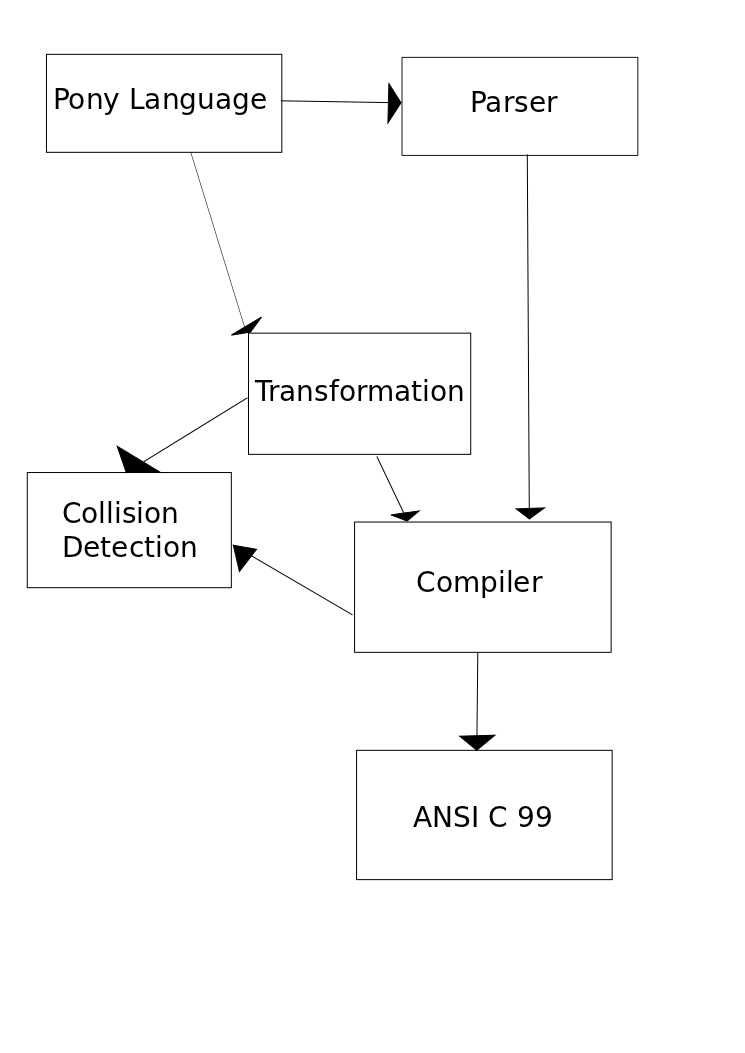
\includegraphics[width=10cm]{./components.png}
\caption{\label{fig:modules}Pony Modules}
\end{figure}

\end{document}
